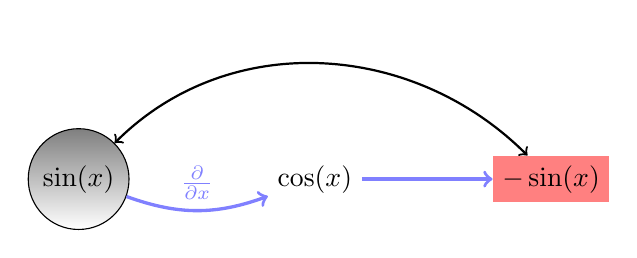
\begin{tikzpicture}
\node (A) at (0,0) [circle,shade,draw] {$\sin(x)$};
\node (B) at (3,0) {$\cos(x)$};
\node (C) at (6,0) [fill=red!50] {$-\sin(x)$};
\draw[->, blue!50, very thick] (A) to[bend right=20]
node[above] {$\frac{\partial}{\partial x}$} (B);
\draw[->, blue!50, very thick] (B) to (C);
\draw[<->, thick] (A) to[out=45, in=135] (C);
\end{tikzpicture}